\section{Cálculo de Pi paralelizado.}

Para el primer apartado probamos a ejecutar en atcgrid.ugr.es el caso más costoso utilizando un solo nodo de cómputo de la máquina, la cuenta acap y la cola acap,
tal y como se nos pide en el enunciado.
Encontramos el resultado en la Figura 1.2.

\begin{figure}[H]
    \centering
    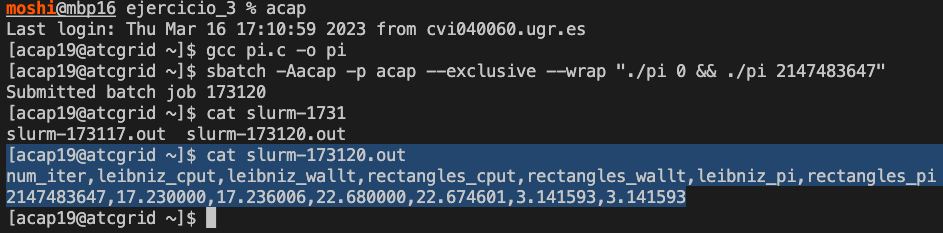
\includegraphics[width=\textwidth]{ej3a.png}
    \caption{Comandos ejecutados para el primer apartado del tercer ejercicio junto a los resultados obtenidos.}
\end{figure}

Para el segundo apartado paralelizamos el cálculo de Pi dividiendo las iteraciones entre todos los procesos.
Buscamos por Internet un \textit{cheatsheet} de MPI, para ver las posibles funciones que podemos utilizar. Vemos que
MPI ofrece mecanismos para la reducción. Seguimos los siguientes pasos, siempre comprobando en cada paso que todo
funciona correctamente.

\begin{enumerate}
    \item Divide la carga de trabajo entre los distintos procesos para el cálculo de Pi por el método de los rectángulos utilizando \texttt{MPI\_Reduce}.
    \item Calcula el tiempo de CPU total y súmalo al global mediante \texttt{MPI\_Reduce}.
    \item Abstrae las funcionalidades del punto 1 y 2 dentro de una función \texttt{evalua}.
    \item Adapta los métodos para el cálculo de Pi a la interfaz \texttt{calcula\_ppi\_t}.
    \item Ejecuta ambos métodos para el cálculo de Pi haciendo uso de la función \texttt{evalua}. 
\end{enumerate}

En el punto 4 modificamos las funciones para que funcionen con la nueva interfaz, que obliga a calcular
dentro de un intervalo. Analizamos cómo funcionan cada uno de los algoritmos e inicializamos el caso base según
el intervalo que se le pida.

\pagebreak

Ejecutamos nuestra versión del algoritmo paralelizado y lo analizamos. Para ello exportamos los datos a un csv y
creamos un gráfico a partir de este, el cual encontramos en la Figura 1.3.

\begin{figure}[H]
    \centering
    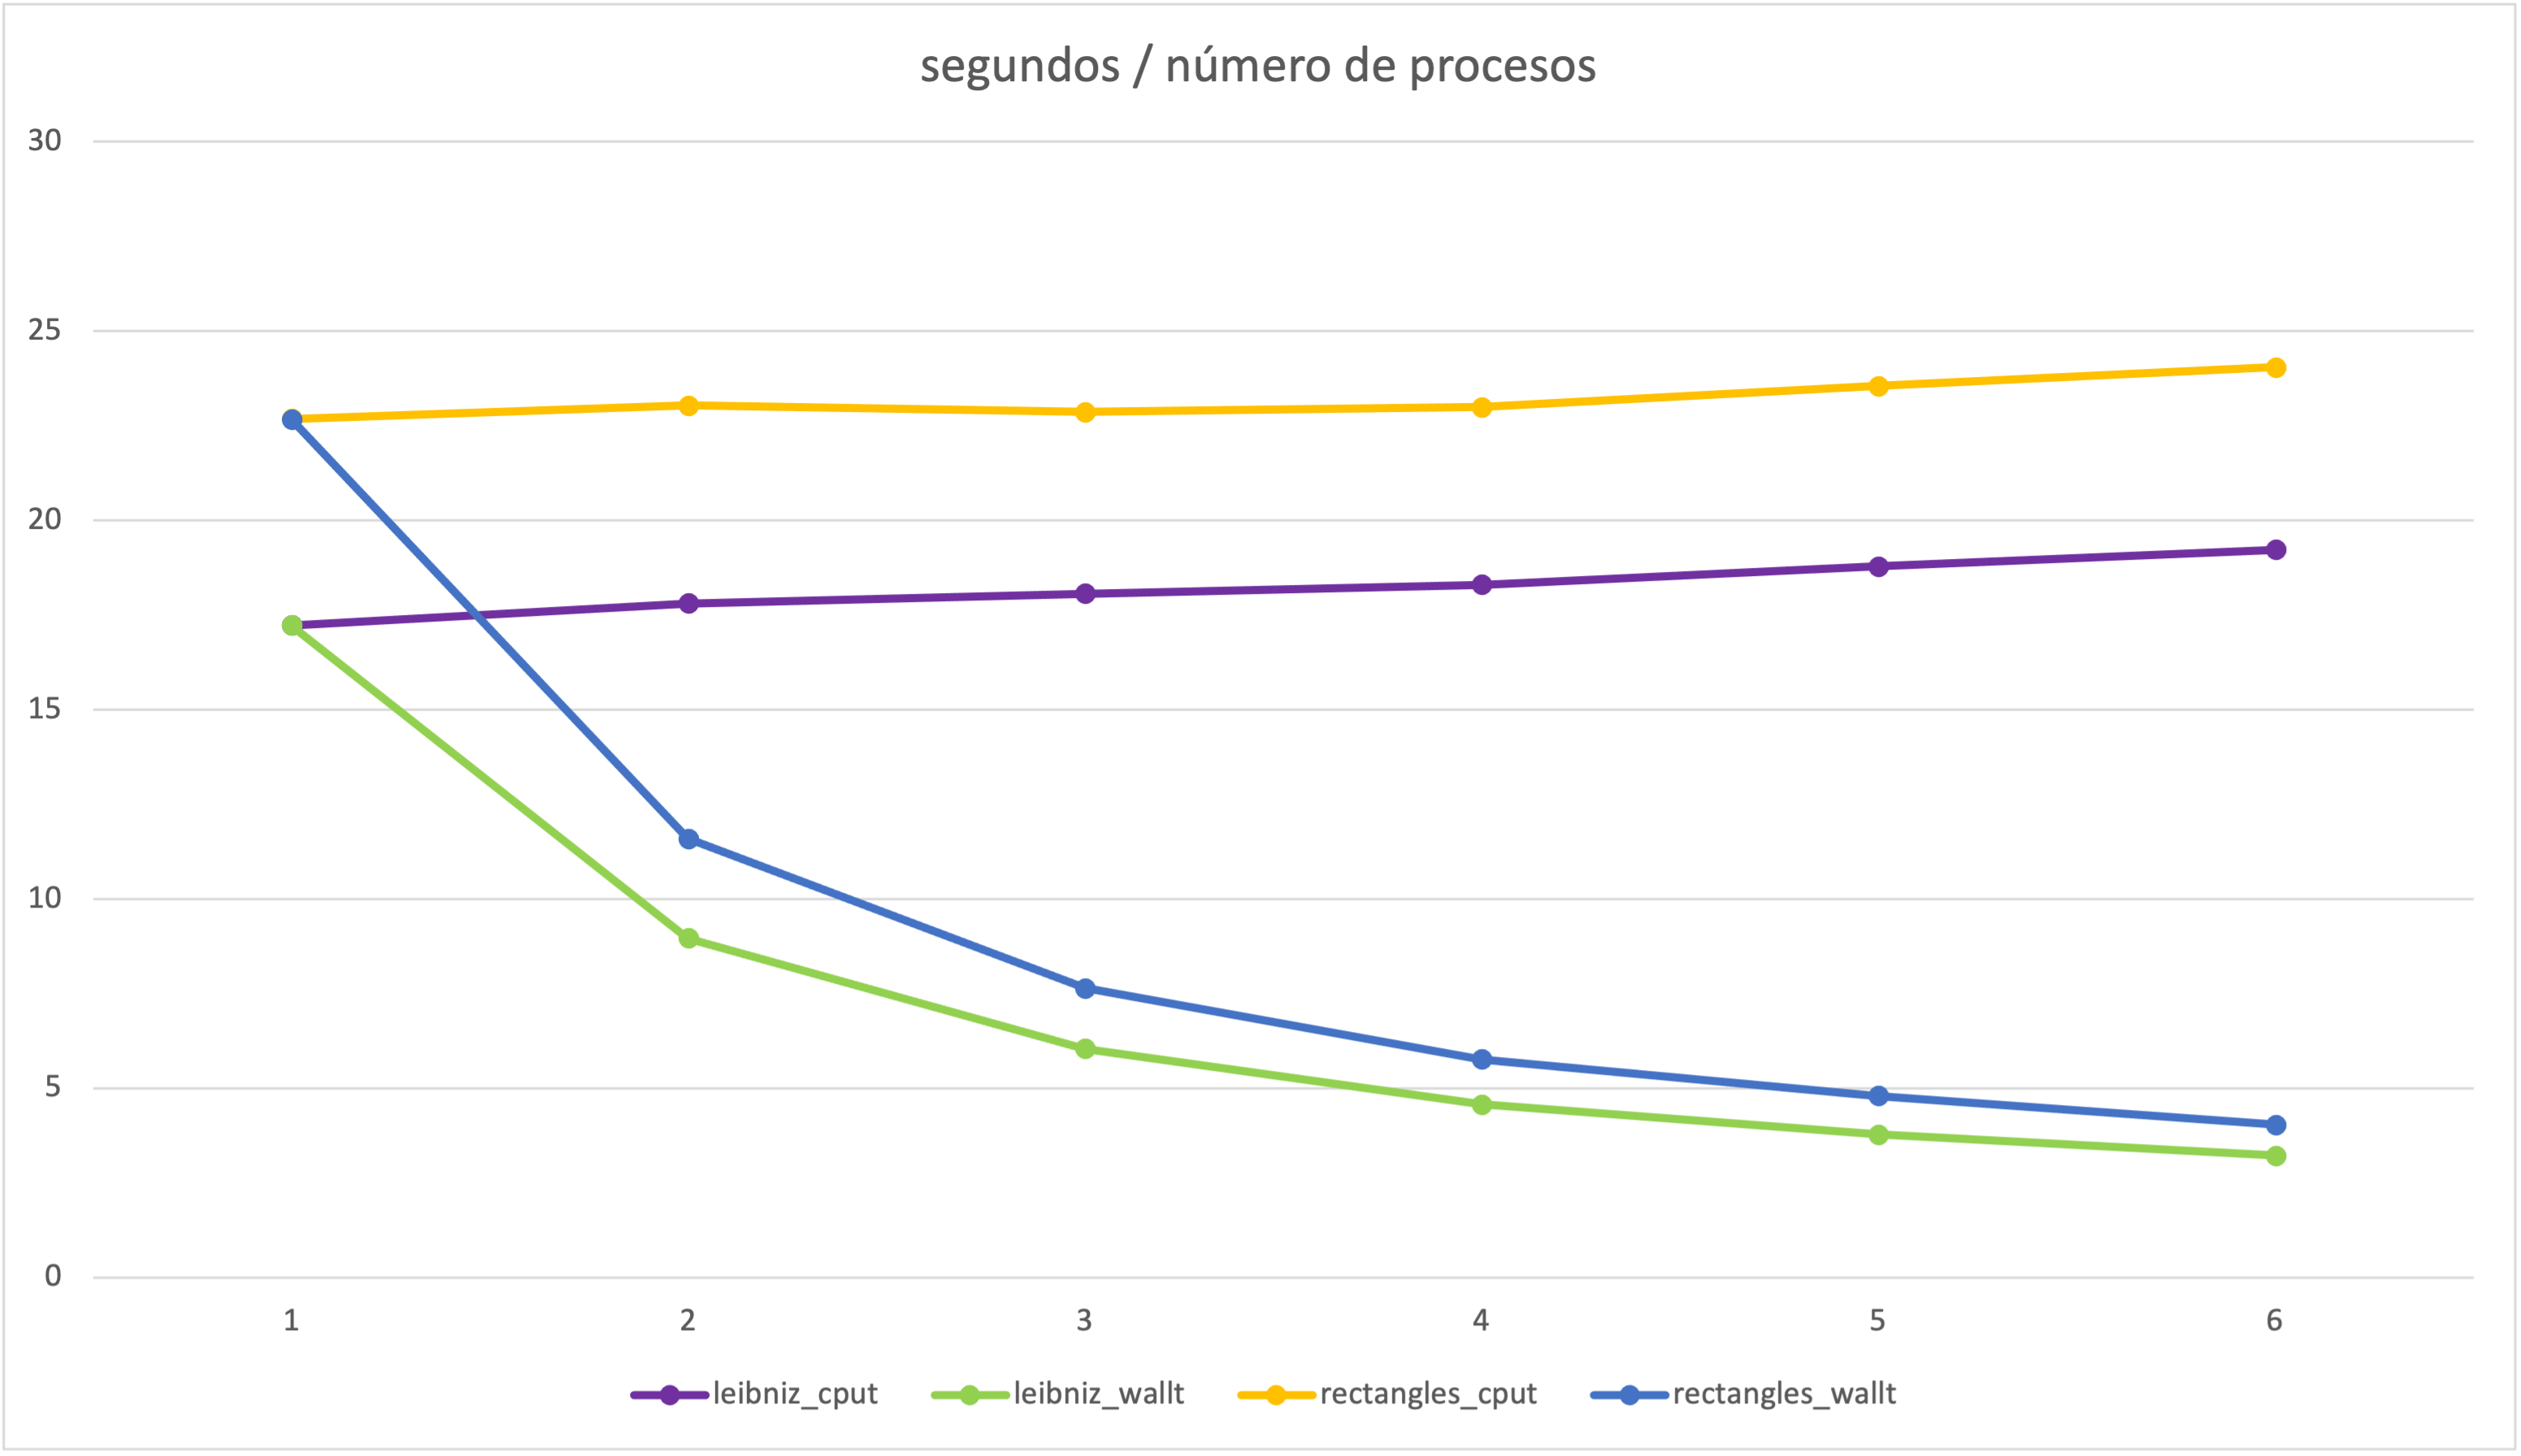
\includegraphics[width=16cm]{ej3b.png}
    \caption{Relación segundos / número de procesos. Observamos que ambos algoritmos tienen tiempos de ejecución
    diferentes, independientemente del número de procesos empleado. También observamos cómo el \textit{wall time}
    decrece progresivamente, mientras que el tiempo de CPU tiende a crecer levemente según se va
    aumentando el número de procesos.}
\end{figure}

\begin{figure}[H]
    \centering
    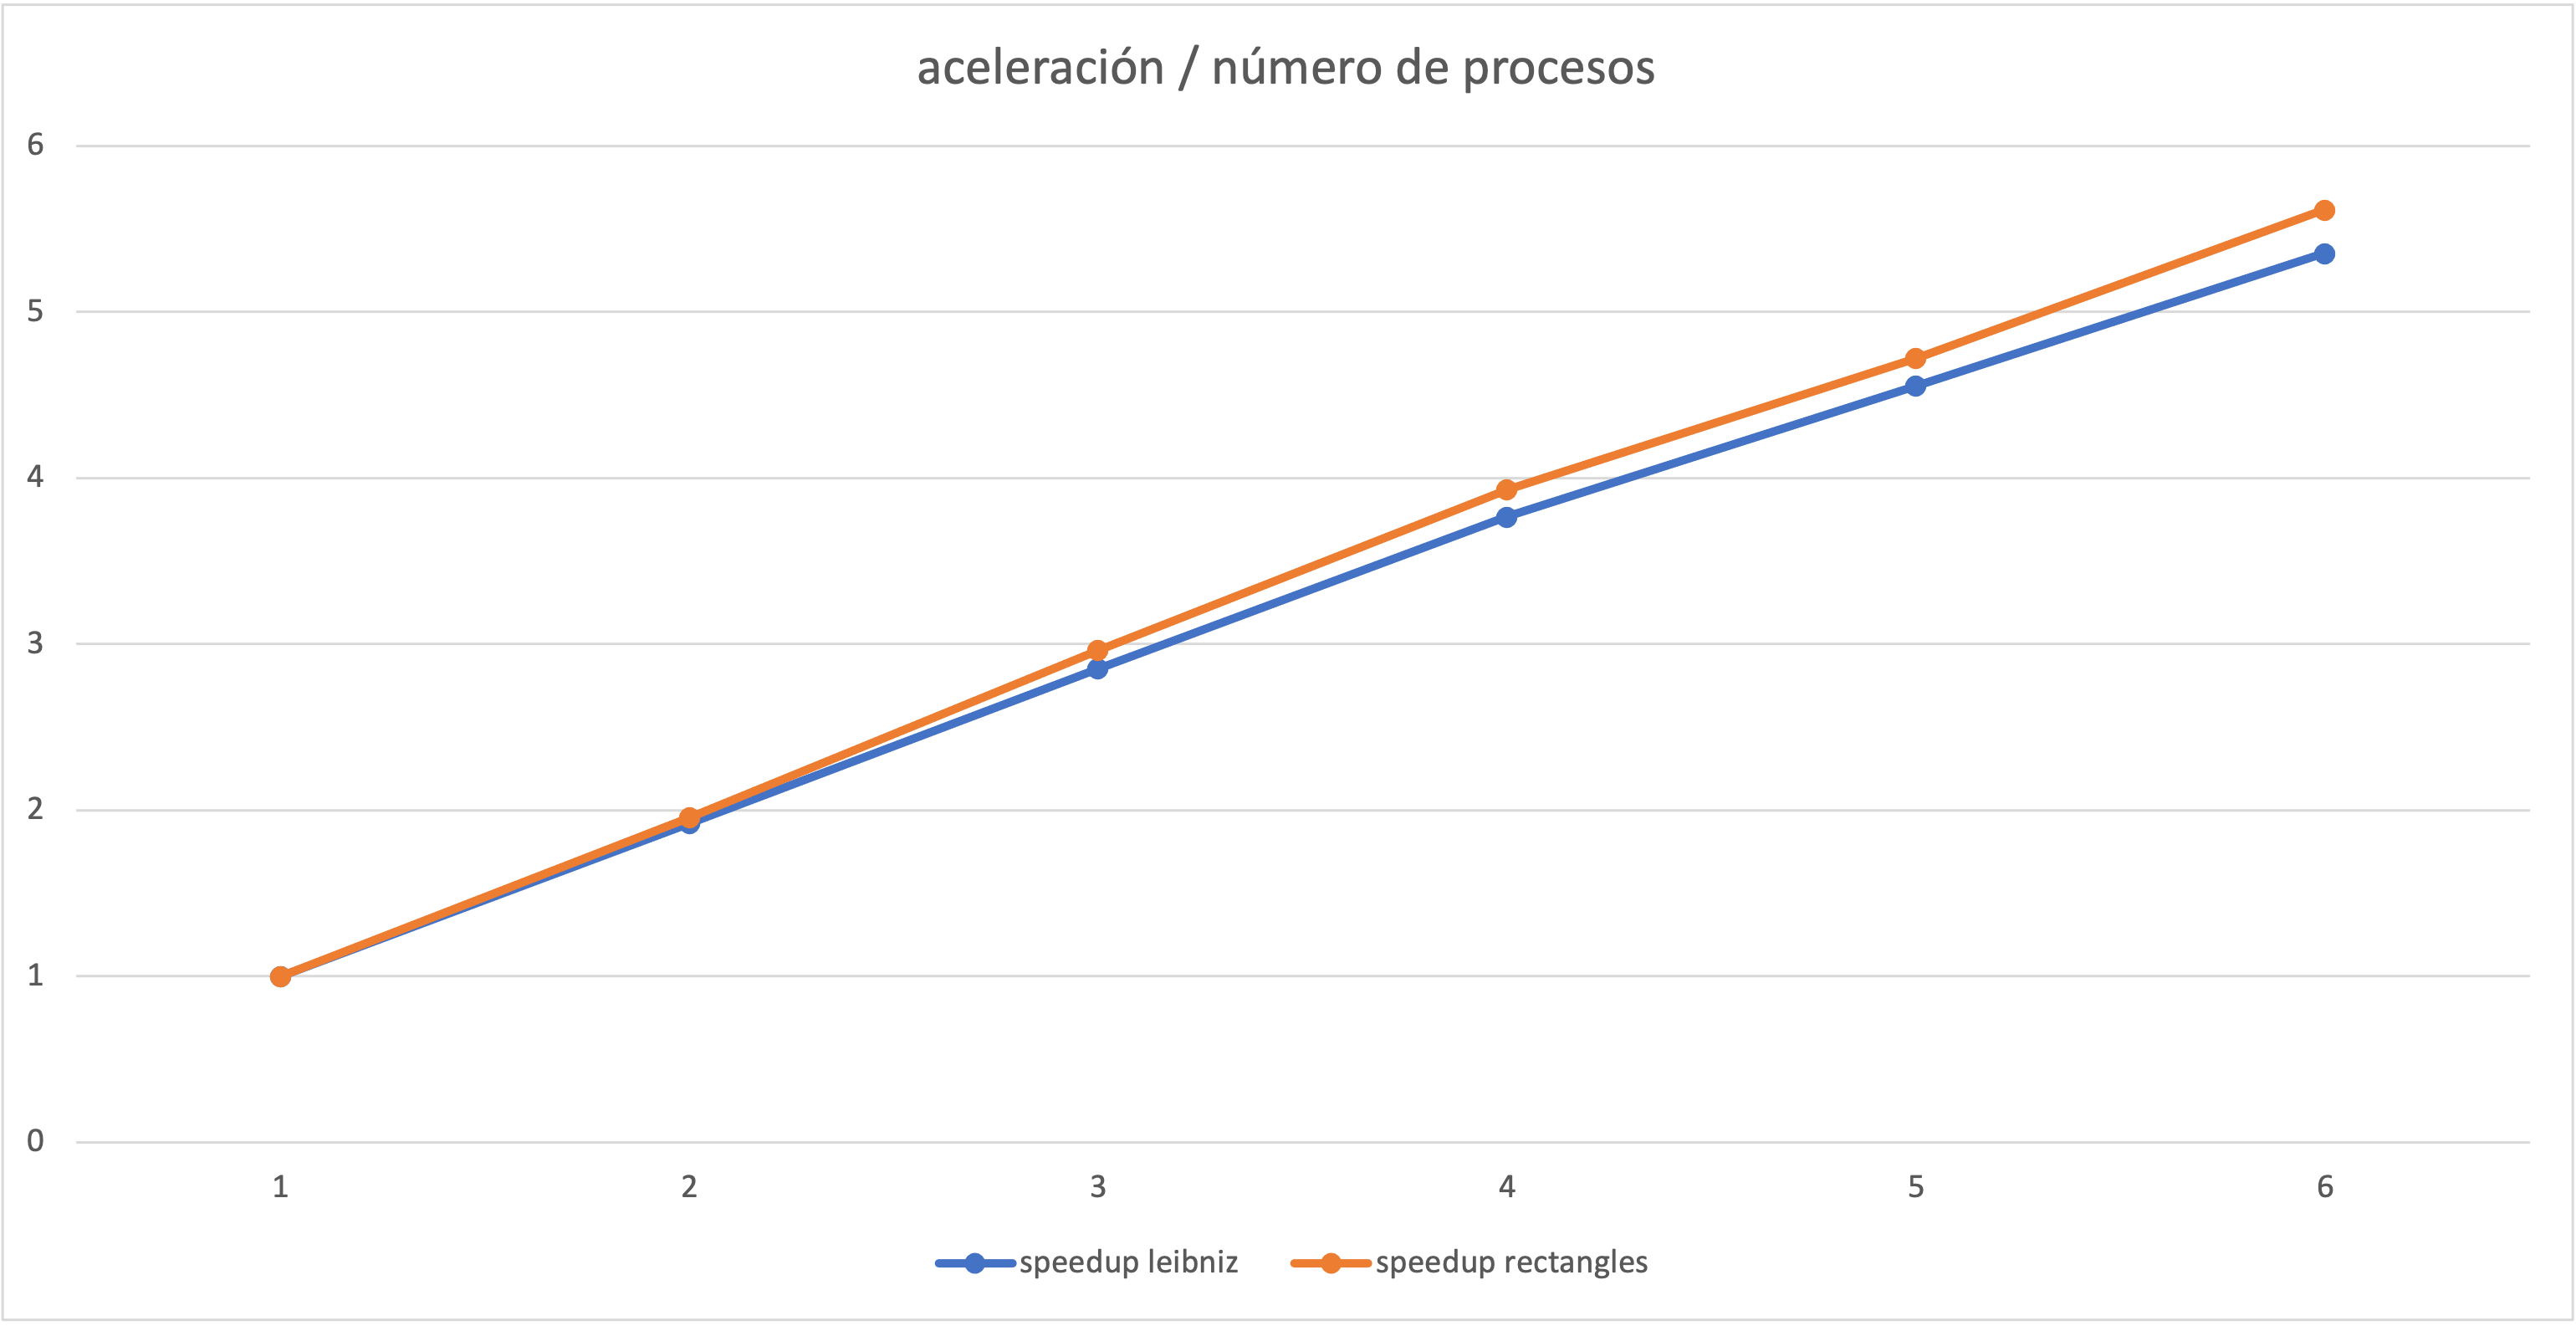
\includegraphics[width=16cm]{ej3c.png}
    \caption{Relación aceleración / número de procesos. Observamos \textbf{para los datos obtenidos} que la aceleración crece linearmente, con una pendiente
    aproximada de 0.9. Esto se debe a que el algoritmo puede ser paralelizado completamente, ya que el cálculo para cada paso
    no depende en ningún otro, únicamente teniendo que sincronizar los distintos procesos al final de este al reducir las sumas locales.}
\end{figure}
